\chapter{Sistemas de Monitorización}

El sistema de monitorización se encarga de recopilar información acerca del estado de los servidores de una infraestructura. Entre las métricas y datos que debe recopilar se encuentran:

\begin{itemize}
    \item \textbf{Estado del servidor}: cantidad de RAM utilizada, estado de los discos duros, carga del servidor, sistema de ficheros,  …
    \item Estado de los \textbf{servicios que tiene el servidor}: servidor web, número de procesos que tiene, bases de datos, conexiones existentes, cola de correos electrónicos para enviar si es un servidor de correo, … Dependiendo del servicio habrá que realizar unas comprobaciones u otras.
    \item \textbf{Infraestructura en la que se encuentran}: estado de la red, conexión a otros servidores, …
    \item \textbf{Estado del clúster}: en caso de que el servidor pertenezca a un clúster, hay que comprobar que el clúster se encuentra en perfecto estado.
    \item \textbf{Dependencias externas}: un servidor puede depender a su vez de otros, o de servicios externos, que deben de estar funcionando de manera correcta.
\end{itemize}

Normalmente en la monitorización actúa un \textbf{agente} (o servicio) instalado en el equipo monitorizado que obtiene la información requerida que se envía a un servidor central que recopila la información de toda la infraestructura monitorizada.

Esta información suele ser almacenada durante un periodo de tiempo determinado (un año, por ejemplo) para poder ser usada y comparar la situación de los servidores a lo largo del tiempo. Gracias a esta comparación temporal \textbf{se puede llegar a predecir el estado del servidor} a unos días/semanas vista y evitar problemas antes de que sucedan (no tener espacio en discos duros, mal funcionamiento de servicios por falta de RAM, … ).

\infobox{\centering\textbf{La monitorización de servicios y equipos dentro de una infraestructura debe considerarse parte del proyecto, ya que es una parte muy importante de cara al mantenimiento del mismo.}}

\section{Monitorización de servidores}
Es habitual que los sistemas de monitorización funcionen en base a plantillas, que posteriormente se pueden asociar a los servidores monitorizados. Estas plantillas contendrán los servicios que deben ser monitorizados en cada tipo de servidor, ya que no es lo mismo monitorizar un servidor web o un servidor con un SGBD.

Para monitorizar un servidor lo habitual suele ser realizar las siguientes operaciones:

\begin{itemize}
    \item \textbf{Comprobar conectividad con el servidor}: suele ser habitual que los servidores estén fuera de nuestra red (en un proveedor de Internet, en un cliente, en otra oficina…), por lo que es necesario que exista conectividad de alguna manera para poder realizar la monitorización. En caso de no estar en nuestra red, el uso de una VPN es lo más utilizado.
    \item \textbf{Instalar un agente en el propio servidor}: Será el encargado de recopilar la información necesaria para mandarla al servidor central. Dependiendo del sistema de monitorización utilizado, necesitaremos un tipo de agente u otro. Algunos se encargan de realizar todas las comprobaciones y otros llaman a otros programas para realizar las comprobaciones y después mandar el resultado al servidor central.
    \item \textbf{Dar de alta el servidor en el sistema centralizado}: Tal como se ha dicho previamente, lo habitual es contar con un sistema centralizado en el que se tendrán todos los servidores y el estado de las comprobaciones realizadas. De ser así, habrá que darlo de alta, y para ello se necesitará:

    \begin{itemize}
        \item \textbf{Nombre del servidor}: Un nombre que a simple vista identifique el servidor. Suele ser habitual poner el nombre del cliente también, y/o el tipo de servicio que preste.
        \item \textbf{IP del servidor}: Para poder realizar la conexión al servidor.
        \item \textbf{Plantillas asociadas}: En caso de utilizar un sistema que utilice plantillas, al dar de alta el servidor se le aplicarán las plantillas necesarias para que realicen todos los checks oportunos. Por ejemplo: plantilla de Servidor Linux + plantilla de Servidor web + Plantilla de MySQL.
        \item \textbf{Puerto de conexión}:  Los agentes de monitorización suelen contar con un puerto que queda a la escucha. Si hemos cambiado el puerto, habrá que indicarlo a la hora de dar de alta.
        \item \textbf{Otras opciones}: Dependiendo del sistema de monitorización se podrán añadir muchas más opciones, como por ejemplo:
        \begin{itemize}
            \item \textbf{Servidores de los que se depende}: Imaginemos que el servidor monitorizado depende a su vez de un router que también está monitorizado. Si el router cae, no llegaríamos al servidor, por lo que realmente es una caída por dependencia, aunque el servidor puede estar funcionando de manera correcta. Esto nos puede permitir crear “árboles de dependencias” de servidores.
            \item \textbf{Periodos de monitorización}: Lo habitual es que un servidor esté monitorizado 24x7, pero quizá nos interese realizar cambios y que sólo se monitorice en unas horas determinadas (quizá el resto del tiempo está apagado).
            \item …
        \end{itemize}
    \end{itemize}
\end{itemize}

\section{Funcionamiento de la monitorización}
Para conocer cómo funciona un sistema de monitorización lo mejor es que tomemos como ejemplo un tipo de servicio que queremos monitorizar. Como ejemplo se puede tomar las comprobaciones que queremos realizar a un SGBD (Sistema Gestor de Bases de Datos).

No será lo mismo realizar la monitorización de un servidor MySQL o de un Oracle, pero las comprobaciones que queremos realizar en ellos deberían ser similares. Vamos a querer realizar la monitorización de las mismas comprobaciones: estado de las tablas en memoria, número de hilos en ejecución, número de \textit{slow\_queries}, …; pero los scripts ejecutados serán distintos.

\infobox{\textbf{La monitorización dependerá del propio servicio que vayamos a monitorizar.}}

A continuación se puede ver el estado de un servidor monitorizado a través del sistema de monitorización \href{https://www.centreon.com/}{Centreon}:

\begin{tcolorbox}[colback=white,title=Servidor monitorizado en Centreon]
  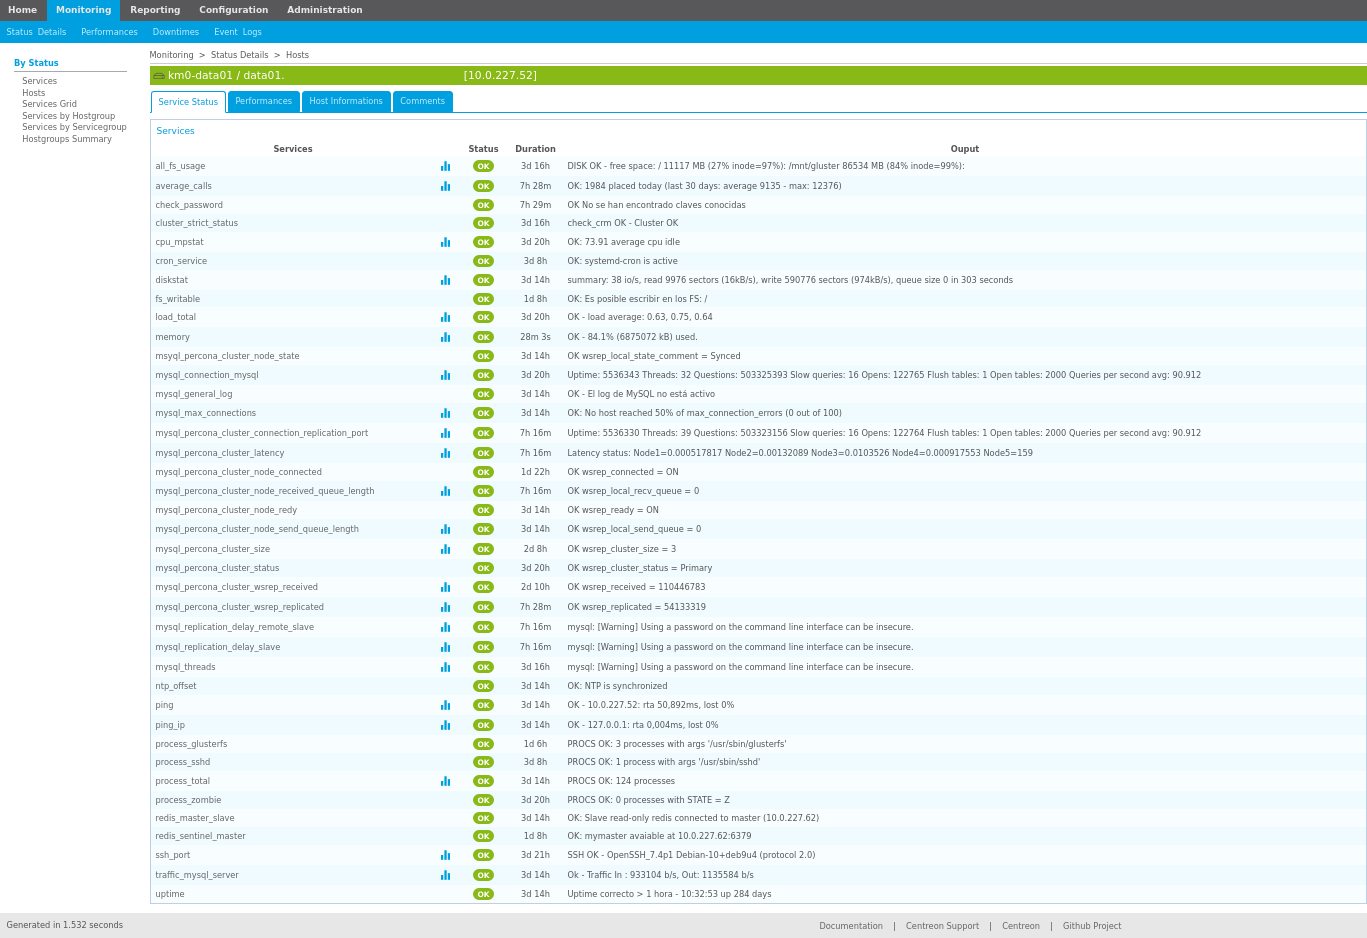
\includegraphics[width=\linewidth]{centreon.png}
\end{tcolorbox}



En la imagen anterior se puede comprobar un número de \textbf{\textit{checks}}, o comprobaciones, que se están realizando sobre un servidor concreto. Cada fila es una comprobación y contienen:

\begin{itemize}
    \item \textbf{Nombre del check/servicio}: Un nombre para identificar qué es lo que se está comprobando con el check.
    \item \textbf{Icono para mostrar gráficas}: Algunos checks recibirán información que puede ser graficada para así poder observar patrones en el comportamiento del servidor. Por ejemplo: cantidad de RAM ocupada, número de procesos en el sistema, número de conexiones a un servidor, …
    \item \textbf{Estado del check}: Normalmente, tras realizar la comprobación, el check termina con uno de los siguientes resultados:
    \begin{itemize}
        \item \textbf{OK}: El resultado obtenido es el correcto.
        \item \textbf{Warning}: El resultado obtenido está entre los márgenes de peligro. Es posible que de seguir así pase al estado siguiente:
        \item \textbf{Crítico}: El servicio devuelve un estado que es considerado crítico, lo que puede hacer que llegue a mal funcionamiento del mismo, o incluso que el servidor comience a dejar de funcionar (imaginemos que el servidor está con el 90\% de la RAM ocupada o de disco duro ocupado).
        \item \textbf{Indeterminado}: Por alguna razón, el \textit{check} no se ha realizado, o el valor devuelto es indeterminado o no se puede saber en qué otro estado situarlo.
    \end{itemize}
    \item \textbf{Duración del estado}: Para conocer cuánto tiempo lleva en el estado la comprobación obtenida. Lo ideal es que nunca haya estados que no sean OK y por lo tanto la duración de los mismos sea lo más alta posible.
    \item \textbf{Valor devuelto por la monitorización}: El valor real devuelto por la comprobación realizada. En base a este resultado se puede realizar las gráficas mencionadas previamente.
\end{itemize}

\infobox{\textbf{El estado del servicio dependerá del valor devuelto por la monitorización.}}

Este resultado se cotejará con los valores que hayamos puesto para que sea considerado OK, Warning o Critical. Es decir, \textbf{en algunos casos el estado del servidor depende de los valores devueltos y de la baremación que le hayamos otorgado}.

Pongamos como ejemplo la monitorización de un SGBD:
\begin{itemize}
    \item \textbf{El servicio del SGBD está funcionando}: Ahí no hay baremación posible. Si el servicio no está arrancado, es lógico pensar que el estado es crítico y que por tanto hay que ver qué ha ocurrido.
    \item \textbf{Número de conexiones en el SGBD}:  El resultado devuelto será un número entero (que podremos graficar para obtener patrones). En este caso, podemos decidir los rangos para que el resultado sea OK, Warning o Critical. Es decir, si el resultado obtenido está por debajo del umbral de Warning, el sistema considerará que el estado es OK. Si está en dicho rango, será Warning y si está en el rango de Critical, así lo indicará.
\end{itemize}

Esta baremación y \textbf{estos rangos} se suelen aplicar también en las plantillas de los servicios. Hay que entender que también \textbf{pueden ser modificados y personalizados para un servidor concreto}. No es lo mismo que un SGBD tenga 500 conexiones simultáneas si tiene 8Gb de RAM o si tiene 128Gb (en el primer servidor se puede considerar que es un estado crítico mientras que en el segundo es lo esperado).

Cuando un \textit{check} termina siendo un Warning o un Critical \textbf{es habitual que haya un sistema de alarmas configurado}. Dependiendo del sistema utilizado, notificará a los administradores mediante e-mail, mensajería instantánea, SMS, … para que realicen un análisis lo antes posible y solucionen el estado del servicio.

\infobox{\textbf{Los sistemas de monitorización suelen contar con un sistema de alarmas para que nos avise de los servicios caídos.}}


\subsection{Monitorización básica}
Tal como se ha comentado, en los servidores se suele realizar una monitorización del estado del mismo que suele ser común para todos, por lo que lo habitual suele ser tener una plantilla genérica para todos los servidores con la que se monitorizará:
\begin{itemize}
    \item Cantidad de RAM utilizada
    \item Cantidad de memoria virtual utilizada
    \item Carga de la CPU
    \item Espacio libre en las unidades de disco duro
    \item Estado del sistema RAID del servidor (en caso de tenerlo)
    \item Cantidad de usuarios conectados a la máquina
    \item Estado de puertos de conexión (SSH, por ejemplo)
    \item Latencia hasta llegar al servidor
    \item …
\end{itemize}

Es cierto que no será lo mismo monitorizar un sistema GNU/Linux o un sistema Windows (ya que puede variar alguno de las comprobaciones a realizar), pero el estado general que queremos conocer es el mismo. Por lo tanto, lo habitual es tener dos plantillas, una específica para servidores Windows y otra para GNU/Linux.

\def\test{sgbd}
\ifx\test\@minititle
  %% THIS PART ONLY IN SGBD BOOK
\subsection{Monitorización de SGBDs}
En el caso que nos ocupa, el de los Sistemas Gestores de Bases de Datos, aparte de la monitorización básica comentada previamente, necesitaremos monitorizar el estado del SGBD propiamente dicho. Para ello, de nuevo, se crearía una plantilla específica para cada SGBD que podamos tener en nuestra infraestructura. No será lo mismo monitorizar un servidor basado en MySQL o un Oracle, aunque muchos checks a comprobar deban ser lo mismo, pero la manera en la que se realizará la comprobación en el servidor será distinta.

Entre las comprobaciones que podemos realizar en un SGBD nos podemos encontrar con:
\begin{itemize}
    \item Servicio SGBD arrancado
    \item Cantidad de RAM utilizada por el SGBD
    \item Número de conexiones a las bases de datos
    \item Número de hilos en ejecución del SGBD
    \item Número de queries en ejecución
    \item Número de tablas en memoria
    \item Número de tablas bloqueadas
    \item …

\end{itemize}

\else
  %% THIS PART IN OTHER BOOKS
\subsection{Monitorización de Servicios}
Aparte de la monitorización básica comentada previamente, necesitaremos monitorizar el estado de los servicios que pueda tener el servidor propiamente dicho. Para ello, de nuevo, se crearía una plantilla específica para cada tipo de Servicio que podamos tener en nuestro servidor.

No será lo mismo monitorizar un servidor que tenga un servidor web, un servidor de base de datos, un proxy… O puede que el servidor cuente con todos esos servicios.

Es por eso que a la hora de realizar la monitorización de un servidor \textbf{es muy importante conocer qué funciones desempeña cada servidor en la infraestructura a la que pertenece} y analizar los servicios que tiene arrancados para posteriormente ser monitorizados.

\infobox{\textbf{Es muy importante conocer qué funciones desempeña cada servidor en la infraestructura a la que pertenece.}}
\fi

\section{Tipos de monitorización}
Existen varias maneras de realizar la monitorización de un servidor, y dependerá del gestor de monitorización que usemos (en caso de usar uno).

Es habitual que cuando nos referimos a sistemas de monitorización lo dividamos en dos grandes familias:
\begin{itemize}
    \item Monitorización Activa
    \item Monitorización Pasiva
\end{itemize}

Estas dos maneras de monitorización suelen ser excluyentes, aunque algunos sistemas de monitorización permiten ambas, por lo que nos puede interesar usar una u otra dependiendo de la situación.


\subsection{Monitorización pasiva}
En la monitorización pasiva el servidor (u objeto monitorizado) es el encargado de mandar la información de manera periódica al servidor central. El agente instalado se ejecutará como una tarea programada cada cierto tiempo (habitualmente unos pocos minutos) e informará de la situación cambiante, de haberla, al servidor central.

Esta manera de monitorización es utilizada también cuando no hay un servidor central. En este caso, si la comprobación ha sido incorrecta, podría mandar un mail al administrador del servidor.

\subsection{Monitorización activa}
Suele ser la manera habitual de proceder de los sistemas que cuentan con un servidor centralizado de monitorización. El servidor de monitorización se encarga de preguntar al servidor, a través de la conexión con el agente, por la comprobación de alguno de los checks, y el agente devuelve la información.

A continuación se puede observar las etapas que existen en un sistema de monitorización activa utilizando un servidor de monitorización central:

\begin{tcolorbox}[colback=white,title=Proceso de monitorización activa]
    \centering
    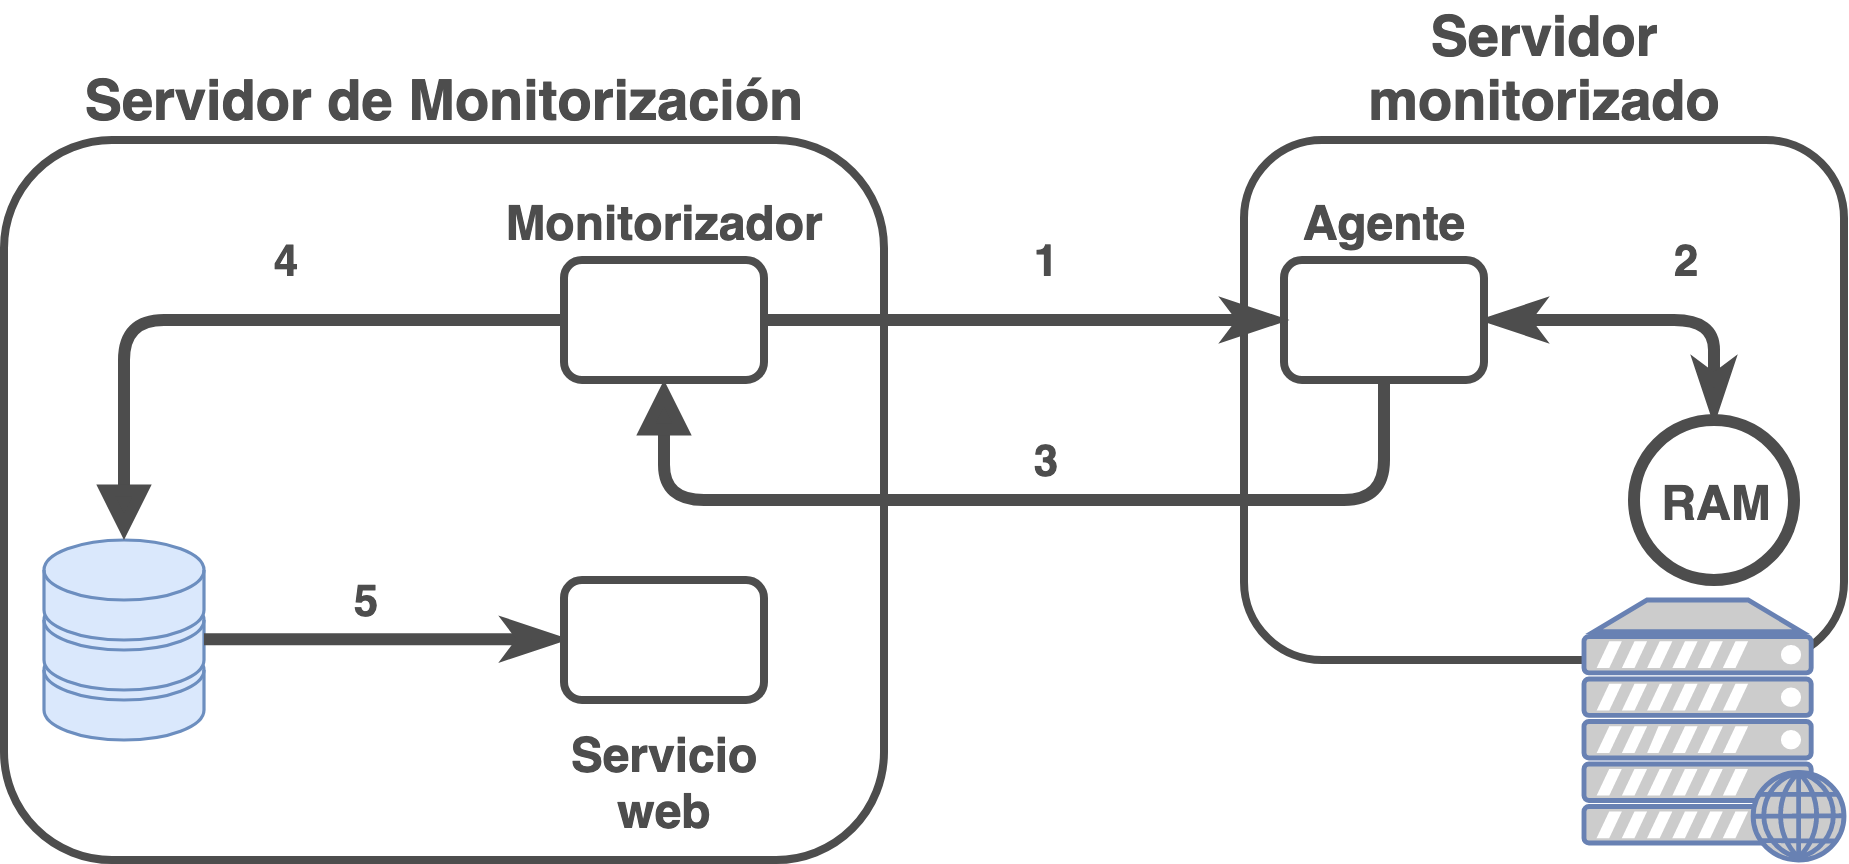
\includegraphics[width=0.6\linewidth]{monitorizacion_activa.png}
\end{tcolorbox}

Las etapas serían:
\begin{enumerate}
    \setcounter{enumi}{-1}
    \item El sistema de monitorización tiene un scheduler (o planificador) que decide cuándo tiene que realizar cada comprobación (normalmente, cada pocos minutos).
    \item El servicio encargado de monitorizar \textbf{establece conexión con el agente remoto} y le pide que compruebe un estado. En este ejemplo se ha optado por la RAM.
    \item El agente en el servidor que se quiere monitorizar recibe la notificación y realiza una \textbf{comprobación local} (normalmente llamando a scripts locales) para obtener la cantidad de RAM ocupada, total y libre que tiene
    \item El agente envía al sistema de monitorización el resultado obtenido en la ejecución de los scripts del paso anterior.
    \begin{enumerate}
        \item El monitorizador al recibir el resultado, lo coteja con los rangos de baremación que tiene y decide si el check está en estado OK, Warning o Critical.
        \item Lo habitual es que si el resultado del servicio no es OK, se ejecute en el servidor de monitorización algún tipo de alarma (ya sea enviar un mail, sistema de mensajería, … ) para notificar a los administradores.
    \end{enumerate}
    \item El sistema de monitorización guarda en una base de datos los resultados obtenidos para así poder realizar posteriores análisis o comprobaciones temporales de los mismos.
    \item Esos datos se suelen visualizar en una interfaz web, tal como hemos visto previamente.
\end{enumerate}

Estos pasos son ejecutados de manera continuada en el servidor de monitorización para cada comprobación que se realiza en cada uno de todos los servidores que se monitorizan. Por lo tanto, se entiende que el propio servidor de monitorización también tiene que ser monitorizado ya que es de vital importancia que su estado sea óptimo.

\subsection{Monitorización centralizada}
Como ya se ha comentado, es el sistema habitual de monitorización. Las ventajas que podemos obtener al hacer uso de este sistema son muchas, pero se pueden destacar las siguientes:
\begin{itemize}
    \item \textbf{Monitorización centralizada}: Aunque parezca obvio, el tener un único sistema en el que concentrar toda la información es muy útil y eficaz.
    \begin{itemize}
        \item La alternativa sería tener una monitorización distinta en cada servidor.
    \end{itemize}
    \item \textbf{Interfaz web}: Hoy en día suele ser habitual que los sistemas de monitorización tengan un servicio web en el que visualizar todos los datos obtenidos.
    \item \textbf{Sistema de plantillas}: De nuevo, es lo habitual, lo que hace que la gestión de monitorización de servidores sea más cómoda.
    \item \textbf{Gestión de usuarios}: Podremos tener usuarios que puedan ver unos servidores u otros, por lo que podemos tener equipos especializados en distintos grupos de monitorización y que sólo se enfoquen en ellos.
    \begin{itemize}
        \item Esto también es útil para dar acceso a los clientes a la monitorización de sus propios servidores.
    \end{itemize}
\end{itemize}

\subsection{Monitorización reactiva}
La monitorización reactiva se puede definir como el sistema de monitorización que no sólo se encarga de comprobar y recibir el estado de los servidores, si no que también reacciona a los mismos para tratar de solucionar los problemas encontrados. Tras esta definición está la idea de que \textbf{existen ciertos fallos recurrentes que no siempre necesitan la intervención humana para solucionarse}, y que por tanto, se puede tratar de ejecutar antes de que sea considerado un problema real.

Como \textbf{ejemplo sencillo} se puede poner \textbf{el espacio libre en disco duro}. Imaginemos que se comprueba que apenas hay espacio en el disco duro de un servidor. En este caso, el sistema de monitorización recibirá que el servidor \textbf{está al 99.95\%} de espacio ocupado, y por tanto, en lugar de notificar a un humano indicando el estado crítico, \textbf{el sistema reacciona de manera automática tratando de liberar espacio}. Se habrá configurado previamente que en la reacción de este error trate de borrar ficheros temporales, vaciar papelera, limpiar ficheros de caché de ciertas rutas … Una vez hecho esto, se volverá a comprobar el estado del servidor. Si el espacio ocupado en disco duro ha bajado y está en modo OK no habrá que hacer nada más, y se habrá evitado que un administrador tenga que realizar dicha tarea. Si por el contrario el estado sigue siendo incorrecto, el sistema notificará el error para que se realice un análisis y se solucione el problema.

Como \textbf{ejemplo extremo} (que no suele ser habitual configurarlo así), imaginemos que \textbf{la RAM consumida por un SGBD es muy alta} y esté poniendo en peligro el estado del servidor, se podría configurar para que \textbf{el sistema reaccione reiniciando el SGBD para que libere la RAM} y vuelva a prestar servicio.


\section{Gestores de monitorización}
Hoy día existen muchos sistemas de monitorización, y dependiendo de nuestras necesidades deberemos optar por uno u otro. A continuación se expondrán varios ejemplos de gestores de monitorización basados en Software Libre, aunque la gran mayoría de ellos cuentan con un sistema dual. Es decir, se puede descargar y montarlo en tu propio servidor o puedes contratar a la empresa para que ellos tengan el servicio central:
\begin{itemize}
    \item \textbf{\href{https://es.wikipedia.org/wiki/Nagios}{Nagios}}: Se puede considerar uno de los sistemas de monitorización más conocidos y del que se han basado otros. Generó mucha comunidad de administradores creando muchos scripts/plugins para hacerlos funcionar con él. Estos mismos scripts suelen ser utilizables en otros sistemas de monitorización.

    \item \textbf{\href{https://www.centreon.com/}{Centreon}}: Originalmente se creó como interfaz web para Nagios, pero poco a poco fue sustituyendo partes de Nagios hasta terminar siendo un sistema de monitorización completo. Existe la posibilidad de realizar la instalación por paquetes, descargar el sistema operativo en una ISO que te instala todo o incluso una máquina virtual con todo ya instalado y con configuración básica. (\href{https://demo.centreon.com/centreon/index.php}{Demo}).

    \item \textbf{\href{https://pandorafms.com/es/}{PandoraFMS}}: Sistema de monitorización creado por el español Sancho Lerena Urrea. Al igual que los anteriores, tiene sistema dual y la instalación se puede realizar por varios métodos.

    \item \textbf{\href{https://www.cacti.net/}{Cacti}}: Sistema más sencillo que los anteriores y habitualmente utilizado sólo en servidores sueltos, es decir, no de manera centralizada.

    \item \textbf{\href{https://munin-monitoring.org/}{Munin}}: Igual que el anterior, ideal para monitorizar unos pocos servidores, ya que no se puede considerar un sistema centralizado como los primeros. Ver \hyperlink{instalar_munin}{anexo de instalación de Munin}.
\end{itemize}

Existen otros sistemas de monitorización basados “en la nube”, cuya funcionalidad es similar a lo expuesto previamente. Para hacer uso de estos sistemas nos descargamos un agente, lo instalamos y se encargará de mandar la información a los servidores de la plataforma contratada. Lógicamente, dependiendo del gasto realizado obtendremos más o menos servicios. Entre este tipo de servicios se pueden destacar:
\begin{itemize}
    \item New Relic
    \item DataDog
\end{itemize}

\def\test{sgbd}
\ifx\test\@minititle
%% THIS PART ONLY IN SGBD BOOK

\section{Monitorizar MySQL}
Todo lo expuesto hasta ahora es referente a los sistemas de monitorización en general, y es similar en todos ellos. Tal como se ha comentado previamente, cuando un servidor cuenta con un servicio éste debe ser monitorizado, y dependiendo del servicio a monitorizar se realizará una serie de comprobaciones u otras.

A la hora de monitorizar un sistema gestor de bases de datos deberíamos tener en cuenta al menos las siguientes comprobaciones, y en el caso de MySQL:
\begin{itemize}
    \item Número de conexiones actuales (usuarios/conexiones tiene el servicio)
    \item Tiempo del servicio activo (uptime)
    \item Número de hilos en ejecución
    \item Tamaño de memoria utilizado
    \item Tamaño de memoria caché utilizado
    \item Número de tablas en memoria
    \item Número de slow queries
    \item Número de conexiones abortadas
    \item Número de queries totales
\end{itemize}

En servidores en alta disponibilidad, deberíamos comprobar, en caso de un clúster:
\begin{itemize}
    \item Número de nodos en el clúster
    \item Estado general del clúster
    \item Latencia entre los nodos del clúster
    \item Si el nodo está conectado al clúster
    \begin{itemize}
        \item  Puede pasar que un nodo “se salga” del clúster (o lo saquemos) para realizar mantenimiento
    \end{itemize}
\end{itemize}

Si el servidor está dentro de una infraestructura de \textbf{Primario → Réplica}:
\begin{itemize}
    \item Estado de la replicación
    \item Retraso de la replicación
    \item Tamaño del binlog
\end{itemize}

Las comprobaciones expuestas son un mero ejemplo, y existen muchas más que podemos realizar a nuestros sistemas. Para poder realizar este tipo de monitorización podemos hacer uso de scripts propios (ya que muchas de las comprobaciones son consultas a variables de estado de MySQL), scripts creados por otras personas o scripts de monitorización hechos de manera exclusiva para MySQL.

\subsection{Scripts propios}
Para realizar gran parte de los checks expuestos previamente se puede hacer uso de scripts propios, ya que pueden realizar consultas de las variables de estado para comprobar y determinar si el estado es correcto.

Un ejemplo de script creado \textit{ad hoc} para nuestro sistema podría ser:

\begin{mycode}{Script propio para monitorizar}{bash}{}
#!/bin/bash
mysql -e "SHOW STATUS LIKE 'Slow_queries';" -N | awk '{print $2}'
\end{mycode}

\subsection{Percona monitoring tools}
La alternativa a hacer uso de scripts propios es usar programas o scripts realizados por terceros, que estén ampliamente probados y que tienen detrás un equipo que quizá sea más amplio que el nuestro, y por tanto esté mejor probado.

La empresa Percona tiene un par de soluciones sobre monitorización de SGBDs (no sólo para MySQL, también para \href{https://www.postgresql.org/}{PostgreSQL} y \href{https://www.mongodb.com/}{MongoDB}), que son:
\begin{itemize}
    \item \href{https://www.percona.com/software/database-tools/percona-monitoring-and-management}{\textbf{Percona Monitoring and Management}}: Un sistema completo de monitorización, interfaz web incluída, que podremos \href{https://www.percona.com/software/pmm/quickstart}{instalar} en nuestros propios servidores. Podemos ver aquí una \href{https://pmmdemo.percona.com/graph/}{demo}.

    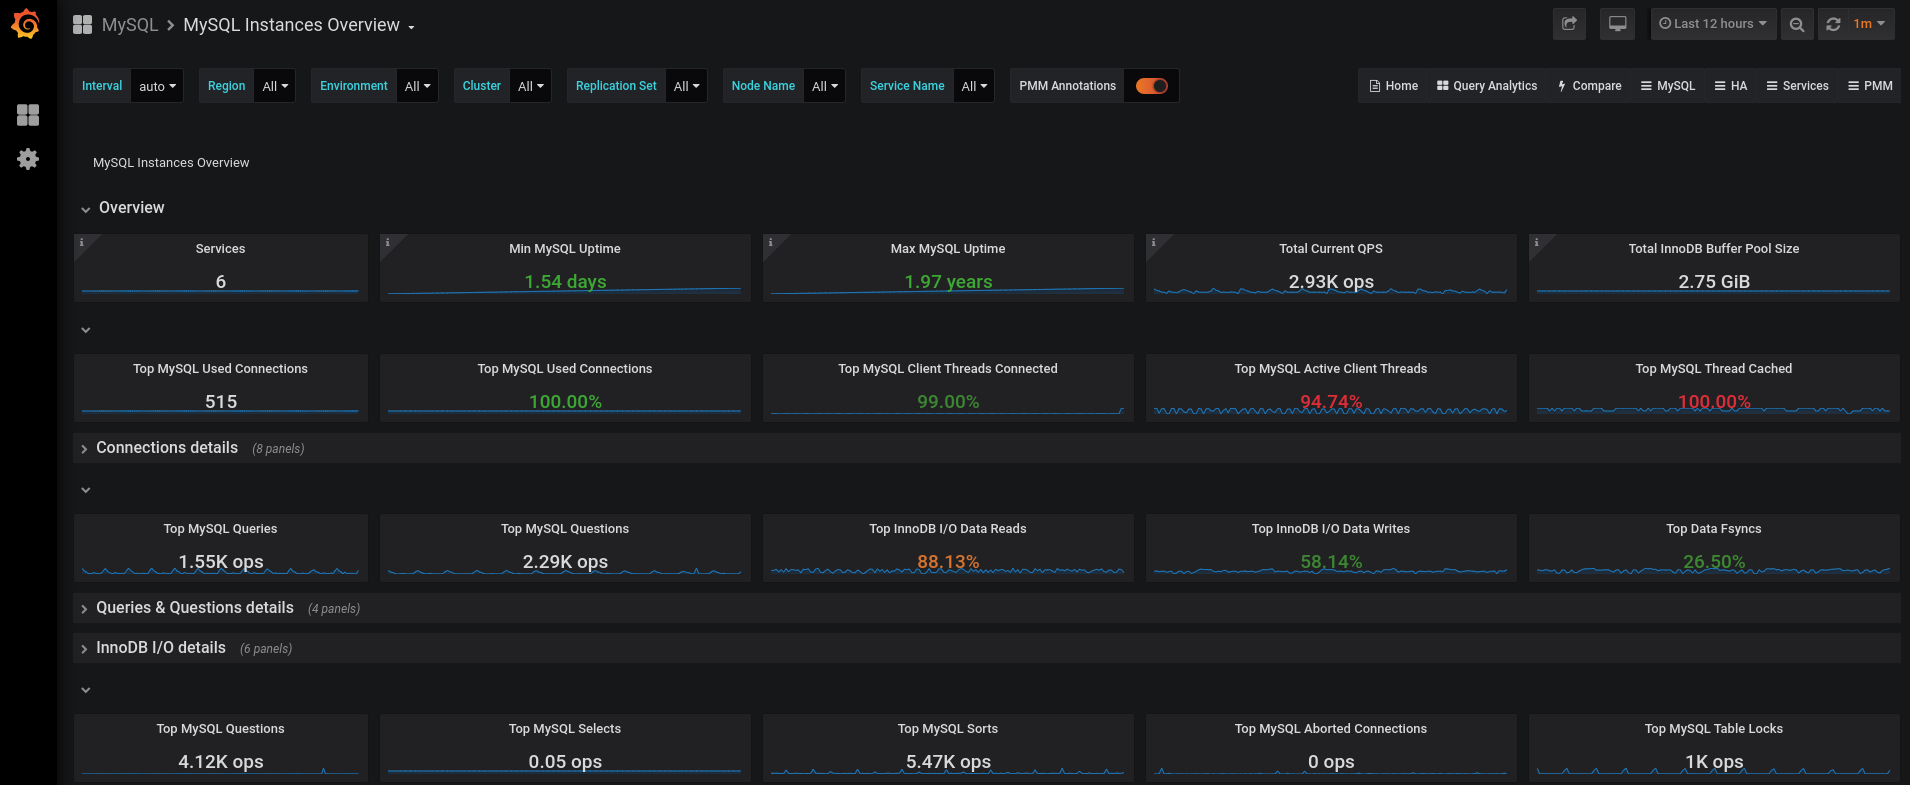
\includegraphics[width=\linewidth]{percona_tools.png}

    \item \href{https://www.percona.com/software/database-tools/percona-monitoring-plugins}{\textbf{Percona Monitoring Plugins}}: En este caso son un conjunto de plugins (o scripts) que podremos utilizar en nuestro sistema de monitorización propio (Nagios, Centreon o Cacti). En la \href{https://www.percona.com/doc/percona-monitoring-plugins/LATEST/index.html}{documentación} explican cómo hacer uso de ellos.
\end{itemize}

\fi

\clearpage